% Compact PGFPlots panel for sampled surface7 BSC bit-scale decomposition.
% Requires \usepackage{pgfplots} and \pgfplotsset{compat=1.18}.
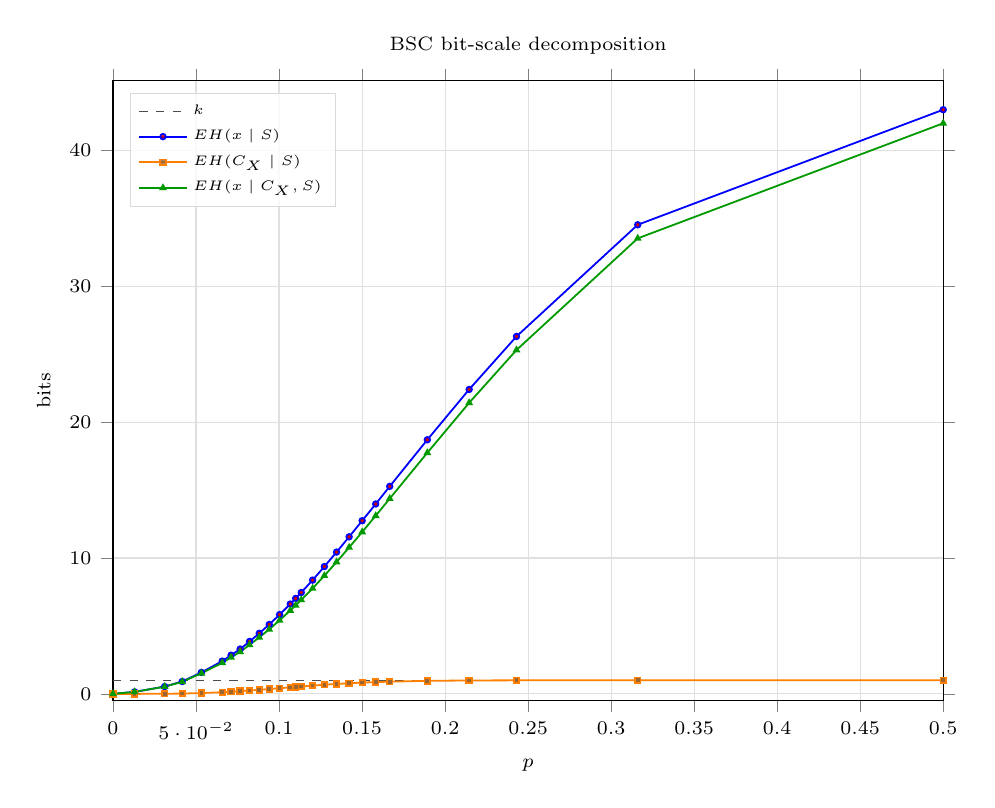
\begin{tikzpicture}
\begin{axis}[
  name=Surface7BSCBitScaleAxis,
  width=\linewidth,
  height=0.78\linewidth,
  title={BSC bit-scale decomposition},
  title style={font=\scriptsize},
  xlabel={$p$},
  ylabel={bits},
  xmin=0, xmax=0.5,
  ymin=-0.5, ymax=45.15,
  grid=both,
  major grid style={black!12},
  minor grid style={black!6},
  tick align=outside,
  tick label style={font=\scriptsize},
  label style={font=\scriptsize},
  legend cell align={left},
  legend style={draw=black!15, fill=white, fill opacity=0.82, text opacity=1, at={(0.02,0.98)}, anchor=north west, font=\tiny},
]
\addplot[black!70, dashed, line width=0.55pt] coordinates {(0,1) (0.5,1)};
\addlegendentry{$k$}
\addplot+[color=blue, mark=*, mark size=1.0pt, line width=0.65pt]
coordinates {(0,0) (0.0129868620555,0.144810740058) (0.0311244603048,0.538078070103) (0.0416926902737,0.911791709061) (0.0532390407768,1.57973254323) (0.0657867063546,2.40982189075) (0.0710958755299,2.84543798127) (0.0765765344037,3.29910088492) (0.0822333323659,3.85790579012) (0.0880715694979,4.4552721398) (0.0940972433461,5.10767327592) (0.100317108961,5.83324971061) (0.106738753821,6.61248020488) (0.110027864438,7.02613786695) (0.113370689941,7.46176021895) (0.120222466333,8.37411512666) (0.127304805976,9.3728507078) (0.134629772869,10.4366462756) (0.142210976498,11.5603506507) (0.150063823499,12.7452515128) (0.158205829694,13.9769814059) (0.166657010397,15.2729682896) (0.189297705371,18.7047427179) (0.21450174486,22.410123898) (0.243003853809,26.3091773595) (0.316019346324,34.5297959056) (0.5,43)};
\addlegendentry{$\mathbb{E}H(x\mid S)$}
\addplot+[color=orange, mark=square*, mark size=1.0pt, line width=0.65pt]
coordinates {(0,0) (0.0129868620555,0.000323855625163) (0.0311244603048,0.00825164588968) (0.0416926902737,0.0239816576268) (0.0532390407768,0.0593398283068) (0.0657867063546,0.123292718259) (0.0710958755299,0.158628007671) (0.0765765344037,0.20303926042) (0.0822333323659,0.247559004964) (0.0880715694979,0.296680183788) (0.0940972433461,0.357154098901) (0.100317108961,0.418915732805) (0.106738753821,0.478789053261) (0.110027864438,0.510171155601) (0.113370689941,0.542440351824) (0.120222466333,0.607560950655) (0.127304805976,0.672900892655) (0.134629772869,0.732107531628) (0.142210976498,0.781568537137) (0.150063823499,0.829946203849) (0.158205829694,0.865996863611) (0.166657010397,0.899049911892) (0.189297705371,0.959189089295) (0.21450174486,0.98681960759) (0.243003853809,0.997383168015) (0.316019346324,0.999968544516) (0.5,1)};
\addlegendentry{$\mathbb{E}H(C_X\mid S)$}
\addplot+[color=green!60!black, mark=triangle*, mark size=1.0pt, line width=0.65pt]
coordinates {(0,0) (0.0129868620555,0.144486884433) (0.0311244603048,0.529826424213) (0.0416926902737,0.887810051434) (0.0532390407768,1.52039271492) (0.0657867063546,2.28652917249) (0.0710958755299,2.6868099736) (0.0765765344037,3.0960616245) (0.0822333323659,3.61034678516) (0.0880715694979,4.15859195602) (0.0940972433461,4.75051917702) (0.100317108961,5.4143339778) (0.106738753821,6.13369115162) (0.110027864438,6.51596671135) (0.113370689941,6.91931986713) (0.120222466333,7.766554176) (0.127304805976,8.69994981514) (0.134629772869,9.70453874401) (0.142210976498,10.7787821135) (0.150063823499,11.915305309) (0.158205829694,13.1109845423) (0.166657010397,14.3739183777) (0.189297705371,17.7455536286) (0.21450174486,21.4233042904) (0.243003853809,25.3117941915) (0.316019346324,33.5298273611) (0.5,42)};
\addlegendentry{$\mathbb{E}H(x\mid C_X,S)$}
\end{axis}
\end{tikzpicture}
